
\section{Studium porównawcze skuteczności wybranych narzędzi STT}
\label{sec:comparative_study}

W niniejszym rozdziale przedstawiono przebieg oraz wyniki eksperymentu badawczego mającego na celu ewaluację jakościową i wydajnościową wybranych systemów rozpoznawania mowy dla języka polskiego. Testy przeprowadzono z wykorzystaniem autorskiej aplikacji badawczej opisanej w rozdziale~\ref{sec:implementation}.

\subsection{Projekt eksperymentu}
\label{subsec:experiment_design}

Eksperyment został zaprojektowany w sposób umożliwiający zweryfikowanie odporności silników ASR na zróżnicowane trudności fonetyczne, leksykalne oraz zakłócenia akustyczne otoczenia.

\subsubsection{Przygotowanie zestawu nagrań}
\label{subsubsec:dataset_preparation}

Materiał badawczy zorganizowano w ustrukturyzowany scenariusz testowy obejmujący 6 nagrań audio przypisanych do trzech głównych kategorii stopnia skomplikowania materiału słownego i warunków nagrania:

\begin{enumerate}
    \item \textbf{Zwykły tekst lektury (warunki czyste):} 
    \textit{Nagranie 1} stanowiło czytany fragment utworu \textit{„Królowa Śniegu”} (Hans Christian Andersen, Rozdział III: \textit{W ogródku wróżki}). Nagranie zrealizowano w cichym pomieszczeniu ze zmiennym tempem wypowiedzi (czytanie wolne, szybkie oraz dynamiczna zmiana tempa w trakcie), co pozwoliło ocenić stabilność modeli przy standardowej mowie ciągłej.

    \item \textbf{Zwykły tekst lektury (warunki zakłócone / hałas):} 
    \textit{Nagranie 2} stanowiło kontynuację tekstu z nagrania pierwszego, jednak zostało zarejestrowane w warunkach znacznego szumu otoczenia (np. pracujący odkurzacz, mikser, głośne rozmowy, muzyka w tle lub szum ruchu ulicznego). Nagranie wykonano z większej odległości mikrofonu od ust ($1$--$1{,}5$~m).

    \item \textbf{Tekst skomplikowany leksykalnie i stylistycznie:}
    \begin{itemize}
        \item \textit{Nagranie 3 (\textit{„Sklepy cynamonowe”}):} Pierwsza strona prozy Bruno Schulza, cechująca się bogatym słownictwem literackim, rzadkimi wyrazami oraz rozbudowaną fleksją języka polskiego.
        \item \textit{Nagranie 4 (Harmonogram i wydarzenia w ZOO we Wrocławiu):} Materiał zawierający specyficzne nazwy własne, egzotyczne nazwy zwierząt oraz liczby i godziny. Test miał na celu weryfikację sposobu zamiany mowy na cyfry (zapis cyfrowy vs. słowny) oraz nazewnictwo specjalistyczne.
        \item \textit{Nagranie 5 (Wierszyki na dykcję / łamańce językowe):} Zestawienie trudnych fraz fonetycznych z zagęszczeniem zbitek spółgłoskowych, służące sprawdzeniu precyzji detekcji trudnych słów polskich.
    \end{itemize}

    \item \textbf{Mowa spontaniczna (wypowiedź swobodna):} 
    \textit{Nagranie 6} miało charakter nieustrukturyzowany ($1$--$3$~minutowa swobodna wypowiedź na dowolny temat, np. opis minionego dnia lub hobby). Celem było przetestowanie radzenia sobie modeli z naturalnymi cechami mowy żywej: pauzami, jąkaniem się, zastanawianiem (\textit{„yyy”}, \textit{„eee”}) oraz wtrąceniami.
\end{enumerate}

\subsubsection{Warunki badania i pomiarów}
\label{subsubsec:test_conditions}

W celu zapewnienia reprezentatywności wyników w zróżnicowanych warunkach użytkowych, przyjęto następujące zasady akwizycji i przygotowania danych:

\begin{itemize}
    \item \textbf{Sprzęt i akustyka:} Nagrania zostały zrealizowane przez wariantywną grupę probantów z użyciem wbudowanych mikrofonów w telefonach komórkowych. Mikrofony znajdowały się w odległości powyżej $30$~cm od ust dla nagrań standardowych oraz $100$--$150$~cm przy nagraniach w hałasie, co wywołało efekt pogłosu i spadku stosunku sygnału do szumu (\textit{ang.~Signal-to-Noise Ratio -- SNR}).
    \item \textbf{Korekta i dopasowanie tekstu wzorcowego (\textit{Ground Truth Alignment}):} Aby uniknąć sztucznego zawyżania błędu WER/CER w sytuacjach, gdy czytający pominął słowo, przejęzyczył się lub nie doczytał fragmentu tekstu, tekst wzorcowy dopasowywano dokładnie do faktycznie wypowiedzianej wypowiedzi. Opracowana aplikacja badawcza automatycznie wyróżniała luki oraz brakujące sekwencje (\textit{diff HTML}), umożliwiając precyzyjną weryfikację tekstru referencyjnego.
    \item \textbf{Normalizacja tekstu:} Przed wyznaczeniem metryk błędu wszystkie teksty referencyjne oraz hipotezy poddawano ujednoliceniu (usunięcie interpunkcji, konwersja do małych liter), co pozwoliło ocenić rzeczywiste dopasowanie leksykalne z wyeliminowaniem różnic w formatowaniu.
\end{itemize}

\subsection{Metryki oceny jakości i wydajności transkrypcji}
\label{subsec:evaluation_metrics}

Do oceny przetestowanych systemów ASR wykorzystano metryki szczegółowo zdefiniowane w części teoretycznej pracy:
\begin{itemize}
    \item \textbf{WER} (\textit{ang.~Word Error Rate}) -- podstawowy wskaźnik dokładności na poziomie słów,
    \item \textbf{CER} (\textit{ang.~Character Error Rate}) -- wskaźnik dokładności na poziomie znaków, szczególnie czuły na polską fleksję i końcówki gramatyczne,
    \item \textbf{RTF} (\textit{ang.~Real-Time Factor}) -- miernik wydajności czasowej:
    \begin{equation}
    \text{RTF} = \frac{T_{\text{processing}}}{T_{\text{audio}}}
    \end{equation}
\end{itemize}

Na potrzeby ewaluacji wszystkie hipotezy oraz teksty referencyjne poddano jednolicie automatycznej normalizacji (sprowadzenie liter do małych, usunięcie znaków interpunkcyjnych i białych znaków) za pomocą funkcji \texttt{normalize\_for\_metrics} z wykorzystaniem biblioteki \texttt{jiwer}.



\subsection{Wyniki testów porównawczych}
\label{subsec:benchmark_results}

W niniejszym podrozdziale przedstawiono ilościowe wyniki badań porównawczych pięciu środowisk rozpoznawania mowy: \textbf{WhisperX} (OpenAI Whisper Large-v3 z dopasowaniem phoneme-level), \textbf{Whisper Offline} (wersja bazowa Large-v3), \textbf{OpenAI GPT-4o Transcribe}, \textbf{Google Cloud Speech-to-Text v2}, \textbf{Microsoft Azure Speech Services} oraz \textbf{Amazon Transcribe}.

Eksperyment objął łącznie około $300$ transkrypcji uzyskanych z nagrań przygotowanych przez 10 probantów, z których każdy zrealizował 6 dedykowanych zadań lektorskich i mówionych zgodnie z ustrukturyzowanym scenariuszem testowym.

\subsubsection{Zbiorczy eksport i przetwarzanie danych pomiarowych}
\label{subsubsec:data_aggregation}

W celu przeprowadzenia rzetelnej analizy statystycznej zbiór surowych wyników zapisanych przez backend w formacie JSON w strukturze katalogowej \texttt{outputs/runs/ID\_RUNU} został scalony do jednolitego arkusza pomiarowego. Przetwarzanie zbiorcze zrealizowano dwutorowo:

\begin{enumerate}
    \item \textbf{Eksport z poziomu interfejsu klienckiego (\texttt{ComparePage}):} Moduł \texttt{compareCsv.ts} umożliwiał bezpośredni eksport bieżących widoków porównawczych ze strony \texttt{compare} do plików w formacie CSV z separatorem średnikowym (\texttt{;}). Eksport obejmował nazwy uruchomień, identyfikatory modeli, wersje, wskaźniki WER i CER, czasy przetwarzania oraz obliczony RTF.
    \item \textbf{Skryptowy eksport zbiorczy (\texttt{json\_to\_csv.js}):} Dedykowany skrypt uruchamiany po stronie backendu rekurencyjnie przeszukiwał katalogi sesji \texttt{outputs/runs}, agregując wszystkie pliki wyjściowe o wzorcu \texttt{transcription\_NAZWA\_MODELU.json}. Skrypt generował zbiorczy plik \texttt{all-results.csv} z separatorami przecinkowymi, wyliczając współczynnik RTF.
\end{enumerate}

\subsubsection{Ogólna dokładność transkrypcji (WER i CER)}
\label{subsubsec:overall_accuracy}

Analiza zagregowanych wskaźników błędu na poziomie słów (\textbf{WER}) oraz znaków (\textbf{CER}) dla pełnego zbioru danych wykazała znaczące rozbieżności w dokładności odwzorowania mowy polskiej pomiędzy testowanymi rozwiązaniami.

\begin{itemize}
    \item \textbf{Współczynnik WER:} Najniższą (najlepszą) średnią wartość wskaźnika WER w całym badaniu uzyskał model \textbf{WhisperX}. Najwyższy błąd na poziomie słów odnotowano dla usługi \textbf{Amazon Transcribe} – średnia wartość WER dla tego dostawcy była o około $75\%$ wyższa w porównaniu do wyniku osiągniętego przez WhisperX.
    \item \textbf{Współczynnik CER:} Najniższą wartość błędu na poziomie znaków zarejestrowano również dla modelu \textbf{WhisperX}. Najwyższym średnim wskaźnikiem CER odznaczał się natywny model \textbf{Whisper Offline} (large-v3) – jego błąd znakowy był o około $120\%$ wyższy względem WhisperX. Główną przyczyną tak wysokiego odchylenia była tendencja bezstanowej implementacji Whisper Offline do generowania halucynacji oraz powielania akapitów przy braku ograniczeń długości nagrania.
\end{itemize}

Wykres~\ref{fig:wer_cer_comparison} przedstawia zbiorcze zestawienie relatywnych wyników dokładnościowych testowanych silników ASR.

\begin{figure}[htbp]
\centering
\begin{tikzpicture}
\begin{axis}[
    ybar=4pt,
    symbolic x coords={WhisperX, GPT-4o, Google, Azure, Amazon, Whisper Off.},
    xtick=data,
    nodes near coords={\pgfmathprintnumber[fixed,precision=0]{\pgfplotspointmeta}},
    nodes near coords align={vertical},
    ylabel={Wskaźnik błędu (\%)},
    ymin=0, ymax=35,
    bar width=12pt,
    enlarge x limits=0.15,
    legend pos=north west,
    x tick label style={rotate=30, anchor=east},
    width=0.95\textwidth,
    height=7cm
]
\addplot coordinates {(WhisperX, 11.4) (GPT-4o, 12.2) (Google, 13.3) (Whisper Off., 16.9) (Azure, 18.0) (Amazon, 19.9)};
\addplot coordinates {(WhisperX, 4.6) (GPT-4o, 4.7) (Azure, 7.6) (Amazon, 7.7) (Google, 8.8) (Whisper Off., 10.1)};
\legend{Średni WER, Średni CER}
\end{axis}
\end{tikzpicture}
\caption{Porównanie wskaźników błędu WER oraz CER dla badanych modeli ASR.}
\label{fig:wer_cer_comparison}
\end{figure}



\subsubsection{Wydajność czasowa i opóźnienia (Real-Time Factor -- RTF)}
\label{subsubsec:performance_rtf}

Pomiar czasu przetwarzania serwerowego (\texttt{compute\_time} / \texttt{rt\_time}) odniesiony do długości nagrania audio (\texttt{audioDuration}) pozwolił na wyznaczenie współczynnika \textbf{RTF} dla każdego modelu.

\begin{itemize}
    \item \textbf{Liderzy wydajności:} Najniższy (najlepszy) wskaźnik RTF osiągnął chmurowy model \textbf{OpenAI GPT-4o Transcribe}, a tuż za nim uplasowała się usługa \textbf{Google Cloud Speech-to-Text v2}. Wyniki te potwierdzają wysoką optymalizację infrastruktury chmurowej pod kątem niskich opóźnień.
    \item \textbf{Najniższa wydajność:} Najwyższy (najgorszy) wskaźnik RTF odnotowano dla lokalnego modelu \textbf{Whisper Offline}. Narzut związany z ładowaniem wag oraz sekwencyjnym dekodowaniem w architekturach o dużej liczbie parametrów powoduje, że modele lokalne wykazują wielokrotnie wyższe opóźnienia niż chmurowe interfejsy API.
\end{itemize}



\subsubsection{Wpływ zakłóceń akustycznych (szum otoczenia)}
\label{subsubsec:noise_impact}

Ocena odporności systemów ASR na zakłócenia obejmowała porównanie nagrań czystych z nagraniami zarejestrowanymi w obecności szumu (np. pracujący odkurzacz, mikser, głośne rozmowy, muzyka w tle) z odległości $1$--$1{,}5$~m od mikrofonu.

\begin{itemize}
    \item \textbf{Pełny zbiór danych:} Wprowadzenie szumu spowodowało istotny wzrost wartości WER we wszystkich badanych modelach. Średni spadek jakości transkrypcji wyniósł około $136\%$, natomiast w skrajnych przypadkach sięgał aż $346\%$.
    \item \textbf{Liderzy odporności na hałas:} W pełnym zbiorze danych najlepsze zachowanie w warunkach zakłóconych wykazują modele \textbf{GPT-4o Transcribe} oraz \textbf{WhisperX}.
    \item \textbf{Najsłabsza odporność:} Usługa \textbf{Microsoft Azure Speech Services} osiągnęła najgorsze wyniki w warunkach hałasu, wykazując wskaźnik WER o około $56\%$ wyższy w porównaniu do GPT-4o (osiągając WER $\approx 0{,}25$).
    \item \textbf{Kontrolowana próbka laboratoryjna (6 nagrań):} W precyzyjnie kontrolowanej próbce nagrań bez błędów czytających hałas o natężeniu zbliżonym do mowy wywołał wzrost WER od $\sim 20\%$ do $\sim 501\%$ (średnio o ok. $200\%$). Najlepsze wyniki osiągnęły \textbf{WhisperX}, \textbf{GPT-4o} oraz \textbf{Amazon Transcribe}, podczas gdy \textbf{Whisper Offline} i \textbf{Azure} były o około $150\%$ gorsze od lidera.
\end{itemize}

 
Wykres~\ref{fig:wer_cer_comparison_noise} przedstawia porównanie błędu WER dla badanych modeli ASR w warunkach czystego tekstu oraz tekstu z hałasem.

\begin{figure}[htbp]
\centering
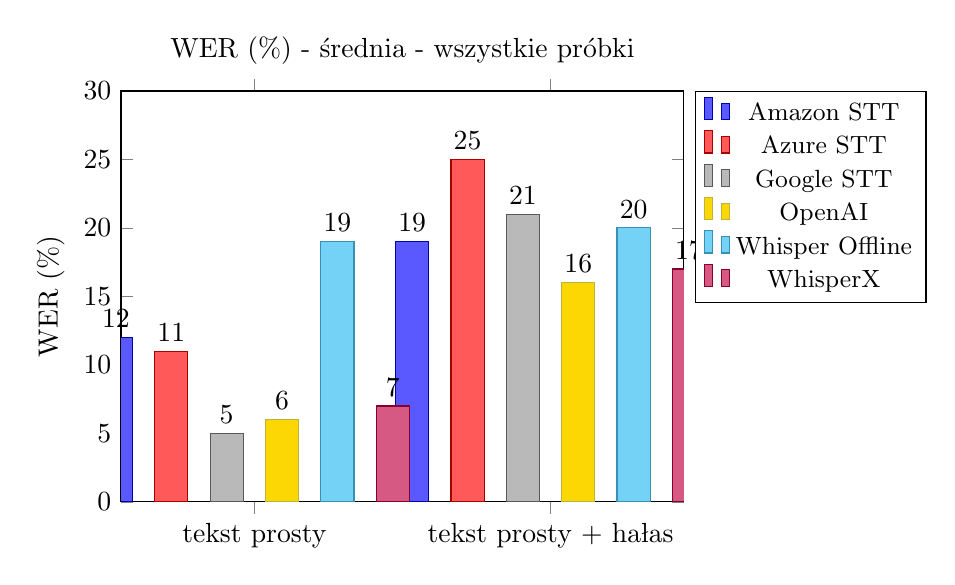
\begin{tikzpicture}
\begin{axis}[
    ybar,
    symbolic x coords={tekst prosty,tekst prosty + hałas},
    xtick=data,
    nodes near coords,
    nodes near coords align={vertical},
    nodes near coords style={
        /pgf/number format/fixed,
        /pgf/number format/precision=0,
    },
    ylabel={WER (\%)},
    ymin=0, ymax=30,
    ytick={0,5,10,15,20,25,30},
    yticklabel={\pgfmathprintnumber[fixed,precision=0]{\tick}},
    ybar=8pt,
    bar width=12pt,
    enlarge x limits=0.45,
    title={WER (\%) - średnia - wszystkie próbki},
    legend style={
        at={(1.02,1)},
        anchor=north west,
        font=\small,
    },
    x tick label style={align=center},
    width=0.72\textwidth,
    height=6.8cm,
]
\addplot[fill=blue!65, draw=blue!65!black] coordinates {
    (tekst prosty,12)
    (tekst prosty + hałas,19)
};
\addplot[fill=red!65, draw=red!65!black] coordinates {
    (tekst prosty,11)
    (tekst prosty + hałas,25)
};
\addplot[fill=gray!55, draw=gray!70!black] coordinates {
    (tekst prosty,5)
    (tekst prosty + hałas,21)
};
\addplot[fill=yellow!75!orange, draw=yellow!70!black] coordinates {
    (tekst prosty,6)
    (tekst prosty + hałas,16)
};
\addplot[fill=cyan!55, draw=cyan!70!black] coordinates {
    (tekst prosty,19)
    (tekst prosty + hałas,20)
};
\addplot[fill=purple!65, draw=purple!70!black] coordinates {
    (tekst prosty,7)
    (tekst prosty + hałas,17)
};
\legend{Amazon STT,Azure STT,Google STT,OpenAI,Whisper Offline,WhisperX}
\end{axis}
\end{tikzpicture}
\caption{Porównanie błędu WER dla badanych modeli ASR w warunkach hałasu.}
\label{fig:wer_cer_comparison_noise}
\end{figure}


\subsubsection{Wpływ specyfiki materiału słownego na jakość transkrypcji}
\label{subsubsec:text_type_impact}

Wartości wskaźnika WER ulegały znacznej zmianie w zależności od stopnia skomplikowania leksykalnego i fonetycznego materiału testowego:

\begin{enumerate}
    \item \textbf{Tekst prosty i mowa swobodna (lektura / wypowiedź nieustrukturyzowana):} Charakteryzowały się najniższym poziomem błędów (średni WER $\approx 0{,}11$). Najlepsze i równorzędne wyniki uzyskały modele \textbf{Google}, \textbf{GPT-4o} oraz \textbf{WhisperX}.
    \item \textbf{Tekst skomplikowany (Schulz, fleksja):} Odnotowano wyższy średni wskaźnik błędu (WER $\approx 0{,}14$). Najwyższą dokładność w tej kategorii wykazała usługa \textbf{Google Speech-to-Text}.
    \item \textbf{Łamańce językowe (zagęszczenie zbitek spółgłoskowych):} Bezapelacyjnym liderem w precyzji rozpoznawania trudnych fraz fonetycznych okazał się model \textbf{WhisperX}.
    \item \textbf{Dane liczbowe i nazwy własne (Harmonogram ZOO Wrocław):} Próbka ta wykazała znaczące rozbieżności formatowania. Modele \textbf{Amazon} i \textbf{Azure} generowały wysoki poziom błędu WER wynikający z mieszanego zapisu godzin (np. słownie \textit{„dziewiąta 50”} zamiast cyfrowego \textit{„9:50”}) oraz błędów segmentacji złożonych nazw własnych.
\end{enumerate}

% todo - wszedzie dodac wykresy zeby sie nie zmarnowaly
\subsection{Analiza jakościowa i statystyczna błędów transkrypcji}
\label{subsec:error_analysis}

O ile wskaźniki WER oraz CER pozwalają na ilościową ocenę dokładności systemów ASR, o tyle pełny obraz ich ograniczeń daje dopiero analiza jakościowa popełnianych błędów. Wykorzystanie zaimplementowanego w aplikacji modułu wizualizacji różnic (\texttt{diff\_html.py}) umożliwiło precyzyjną identyfikację oraz skategoryzowanie mechanizmów zniekształceń.

Przeanalizowany materiał badawczy pozwolił na wyróżnienie czterech głównych klas błędów występujących w testowanych silnikach ASR dla języka polskiego.

\subsubsection{Zjawiska fonetyczne i substytucje zbliżonych słów}
\label{subsubsec:phonetic_errors}

Najczęstszą przyczyną błędów w tekstach lektorskich i mówionych były substytucje fonetyczne, wynikające z bliskości artykulacyjnej poszczególnych głosek języka polskiego:

\begin{itemize}
    \item \textbf{Denazalizacja samogłosek nosowych:} Obserwowano powszechną tendencję modeli do zastępowania samogłoski nosowej \textit{„ę”} sekwencją \textit{„en”}. Przykładem jest transkrypcja wyrazu \textit{„cętkowane”} jako \textit{„centkowane”} (model OpenAI GPT-4o Transcribe). Mimo że z punktu widzenia fonetyki mowy żywej wymowa ta bywa zbliżona, z punktu widzenia algorytmu Levenshteina generuje to błąd substytucji na poziomie słowa.
    \item \textbf{Ubezdźwięcznienia:} Występowało zastępowanie spółgłosek dźwięcznych ich bezdźwięcznymi odpowiednikami (np. zmiana \textit{„b”} na \textit{„p”}). W próbce prozy lektorskiej zarejestrowano zamianę słowa \textit{„izdebki”} na \textit{„izdepki”}.
    \item \textbf{Subsytucje:} W warunkach zakłóconych (nagranie z szumem AGD/muzyki i większej odległości mikrofonu) nawet zaawansowane modele generowały hipotezy całkowicie odległe znaczeniowo od oryginału, dopasowując słowa wyłącznie na podstawie zbliżonego konturu intonacyjnego. W transkrypcji z modelu WhisperX odnotowano m.in. zamiany:
    \begin{itemize}
        \item \textit{„bosymi nóżkami”} $\rightarrow$ \textit{„posyła puszczami”},
        \item \textit{„biegła co tchu po twardej”} $\rightarrow$ \textit{„jego co długo trwa w tej”},
        \item \textit{„cierpkie”} $\rightarrow$ \textit{„ciemnie”}.
        \item \textit{„krople"} $\rightarrow$ \textit{„kotle"}.
        \item \textit{„wykrzywiały"} $\rightarrow$ \textit{„wytrzymiały"}.
    \end{itemize}
\end{itemize}

\subsubsection{Transkrypcja danych liczbowych i formatowanie godzin}
\label{subsubsec:numeric_errors}

Test przeprowadzony na materiale obejmującym harmonogram wydarzeń w ZOO we Wrocławiu ujawnił kluczową słabość niektórych rozwiązań komercyjnych w zakresie standaryzacji tekstu (\textit{ang.~Inverse Text Normalization -- ITN}):

\begin{itemize}
    \item \textbf{Niespójność formatowania godzin (Azure STT i Amazon Transcribe):} Podczas gdy modele Google oraz Whisper rozpoznawały godziny w formacie cyfrowym (np. \textit{„9:30”} lub \textit{„09:30”}), usługi Microsoft Azure i Amazon Transcribe stosowały niespójny zapis mieszany lub czysto słowny. 
    \item Zamiast zapisu \textit{„9:50”} model Azure generował ciąg \textit{„dziewiąta 50”}, a dla godziny \textit{„10:20”} – \textit{„dziesiąta 20”}. 
    \item Z punktu widzenia oceny jakościowej rozpoznanie fonetyczne było poprawne, jednak brak ujednolicenia formatu wywołał sztuczny, drastyczny skok wskaźnika WER (algorytm traktował zapis słowny jako 2 odrębne substytucje względem cyfrowej referencji).
\end{itemize}

\subsubsection{Segmentacja wyrazów i rozpoznawanie nazw własnych}
\label{subsubsec:segmentation_errors}

W nagraniach zawierających specyficzne nazwy własne oraz egzotyczne pojęcia (harmonogram ZOO) silniki ASR wykazywały poważne problemy z wyznaczaniem granic słów (\textit{ang.~word segmentation}):

\begin{itemize}
    \item \textbf{Zniekształcenia rzadkich słów:} Nazwa gatunkowa \textit{„mangaby”} została zinterpretowana przez Azure jako \textit{„maby”}.
    \item \textbf{Błędy scalania i segmentacji fraz:} Fraza \textit{„zoo za mostkiem”} została błędnie scalona do postaci \textit{„zookiem”} lub zmieniona na \textit{„zoologomostkiem ”}, natomiast sekwencja \textit{„czarnoszyje na stawie”} przyjęła postać \textit{„czarno szyje nastawię”}.
\end{itemize}

\subsubsection{Halucynacje, pętlenie i uszkodzenia strumienia}
\label{subsubsec:hallucinations_deletions}

Najcięższe błędy strukturalne odnotowano przy analizie skrajnych przypadków testowych (długie nagrania, pauzy w mowie oraz trudne frazy phonetyczne w łamańcach językowych):

\begin{itemize}
    \item \textbf{Halucynacje i pętlenie (Whisper Offline):} Natywna implementacja modelu Whisper Large-v3, pozbawiona wstępnej filtracji ciszy za pomocą modułu VAD (\textit{ang.~Voice Activity Detection}), wykazuje tendencję do zapętlania się oraz halucynowania na długich pauzach i szumach otoczenia. W analizowanym materiale autoregresywny dekoder po napotkaniu fragmentów bez mowy powielał wygenerowane wcześniej sekwencje i tworzył nadmiarowe akapity tekstu nieobecne w oryginalnym nagraniu (duże bloki insercji).
    \item \textbf{Pominięcia tekstu i znaki obcych alfabetów (Google STT):} W próbie łamańców językowych o bardzo gęstej artykulacji w modelu Google Cloud Speech-to-Text v2 zaobserwowano sporadyczne całkowite pomijanie złożonych sekwencji wyrazowych (\textit{ang.~deletion errors}). Ponadto w skrajnych przypadkach model wstawiał w miejsce nierozpoznanej frazy pojedyncze znaki pochodzące z obcych alfabetów, co wskazuje na błędy w dekodowaniu tokenów przy braku pewności klasyfikatora.
\end{itemize}
% dotąd sprawdzone

\subsection{Wnioski z badań}
